\section{Adaptive Neural Trees}
We now formalise the definition of Adaptive Neural Trees (ANTs), which are a form of DTs enhanced with deep, learned representations. We focus on supervised learning, where the aim is to learn the conditional distribution $p(\mathbf{y}|\mathbf{x})$ from a set of $N$ labelled samples $(\mathbf{x}^{(1)}, \mathbf{y}^{(1)}), ..., (\mathbf{x}^{(N)}, \mathbf{y}^{(N)}) \in \mathcal{X} \times \mathcal{Y}$ as training data.
%ANTs provide a general framework for combining DTs and DNNs of ANTs and subsumes prior work in this subject \cite{rota2014neural,kontschieder2015deep,frosst2017distilling} as specific cases.

\begin{figure}[ht]
	\centering
	\begin{subfigure}[]{0.45\linewidth}
		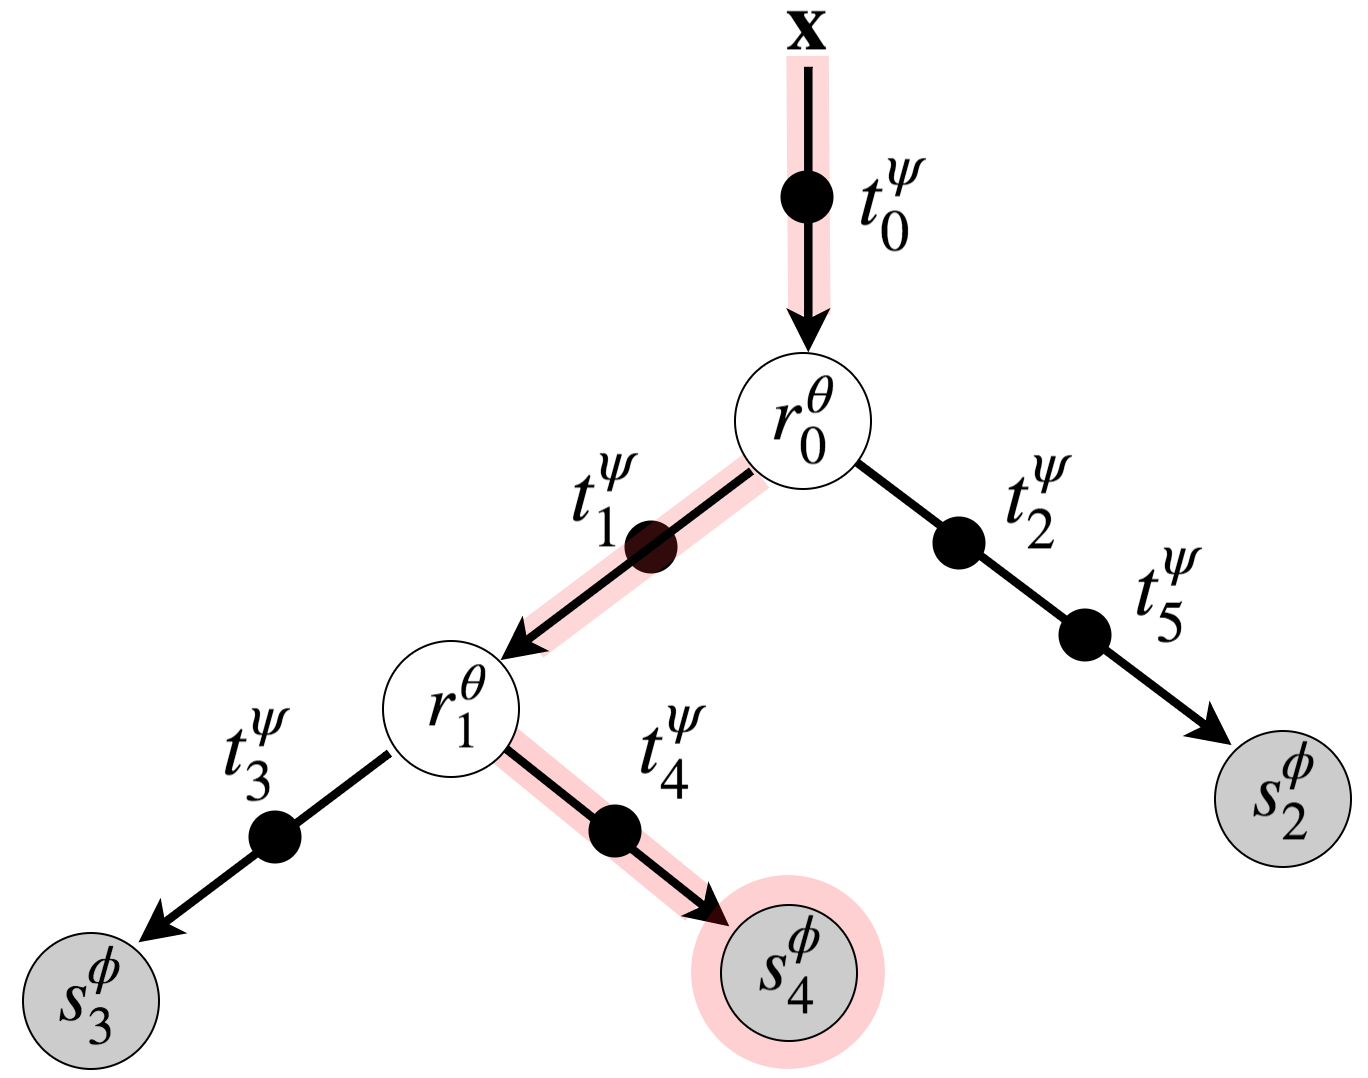
\includegraphics[width=\linewidth]{chapter_7/figures/fig_4_3.png}
	\end{subfigure}
	\hspace{1mm}
	\begin{subfigure}[]{0.52\linewidth}
		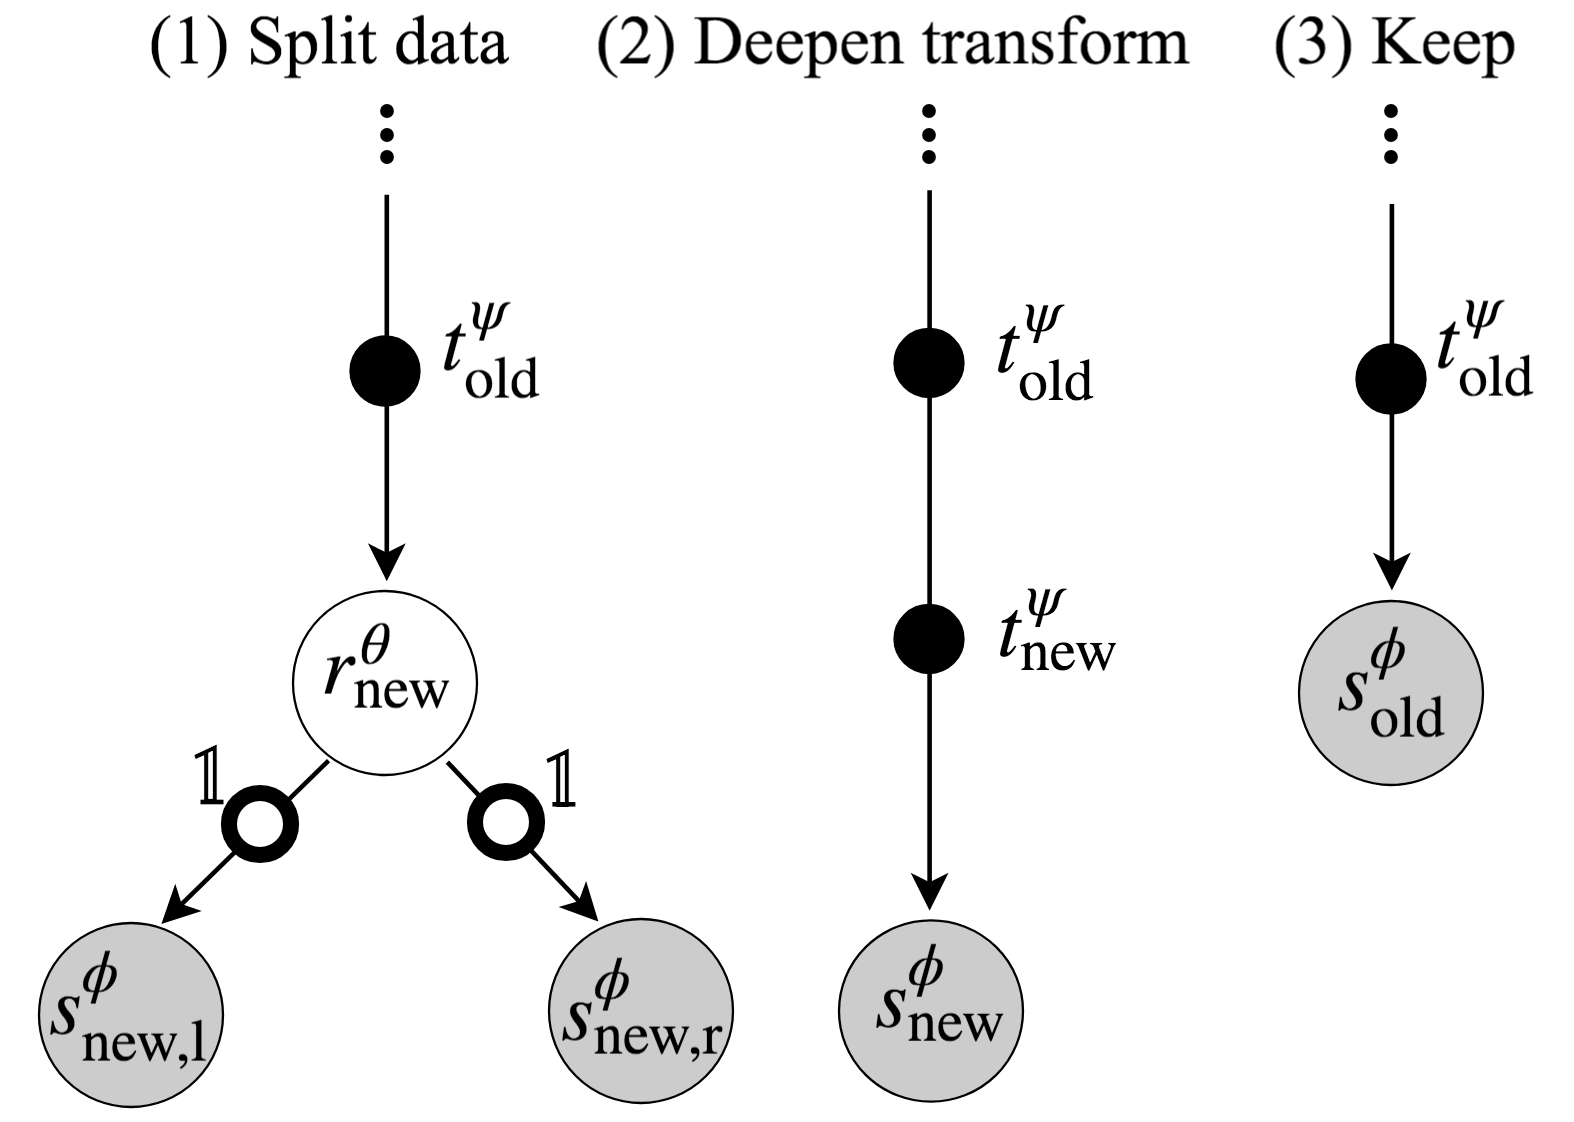
\includegraphics[width=\linewidth]{chapter_7/figures/fig_5_6.png}
	\end{subfigure}
	\caption{\footnotesize \textbf{(Left).} An example ANT. Data is passed through transformers (black circles on edges), routers (white circles on internal nodes), and solvers (gray circles on leaf nodes). The red shaded path shows routing of $\mathbf{x}$ to reach leaf node $4$. Input $\mathbf{x}$ undergoes a series of selected transformations $\mathbf{x}\rightarrow \mathbf{x}^{\boldsymbol{\psi}}_0:=t^{\boldsymbol{\psi}}_0(\mathbf{x})\rightarrow \mathbf{x}^{\boldsymbol{\psi}}_1:=t^{\boldsymbol{\psi}}_1(\mathbf{x}^{\boldsymbol{\psi}}_0) \rightarrow \mathbf{x}^{\boldsymbol{\psi}}_4:=t^{\boldsymbol{\psi}}_4(\mathbf{x}^{\boldsymbol{\psi}}_1)$ and the solver module yields the predictive distribution $p_{4}^{\boldsymbol{\phi}, \boldsymbol{\psi}}(\mathbf{y}):= s^{\boldsymbol{\phi}}_4(\mathbf{x}^{\boldsymbol{\psi}}_4)$. The probability of selecting this path is given by $\pi_{2}^{\boldsymbol{\psi}, \boldsymbol{\theta}}(\mathbf{x}) := r_{0}^{\boldsymbol{\theta}}(\mathbf{x}^{\boldsymbol{\psi}}_0)\cdot(1-r_{1}^{\boldsymbol{\theta}}(\mathbf{x}^{\boldsymbol{\psi}}_1)).$ \textbf{(Right).} Three growth options at a given node: \textit{split data, deepen transform} \& \textit{keep}. The small white circles on the edges denote identity transformers.}
	\label{fig:hierarchy}
\end{figure}

%In this section, we present generalised neural decision trees (ANTs), a form of DTs enhanced with deep, distributed representations. ANTs provide a general framework for combining DTs and NNs, and subsumes prior work in this subject \cite{rota2014neural,kontschieder2015deep} as specific cases. Combined with the optimisation procedure proposed in section \ref{sec:learning}, we will see that ANTs can leverage the differing benefits of the two approaches.
% TODO: Introduce decision trees using the formalism used in the DANT section. Use the DANT section to show the generalisation we introduce.

%a form of decision tree enhanced with deep distributed representation and an efficient mechanism for learning its architecture. The generality of ANTs subsumes the prior work \cite{rota2014neural,kontschieder2015deep,ioannou2016decision} on combining decisions tree and neural networks as specific cases (mode details in section \ref{sec:relatedwork}) and enables to fully leverage the differing benefits of the two approaches. 
%A key difference is the inclusion of transformation operation which enables the representation learning through a series of simple non-linear transforms applied to the input data over the course of traversal down the tree. 
\subsection{Model Topology and Operations}
In short, an ANT is a tree-structured model, characterized by a set of hierarchical partitions of the input space $\mathcal{X}$, a series of nonlinear transformations, and separate predictive models in the respective component regions. More formally, we define an ANT as a pair $(\mathbb{T}, \mathbb{O})$ where $\mathbb{T}$ defines the model topology, and $\mathbb{O}$ denotes the set of operations on it. 

\begin{table}[ht]
	\caption{\footnotesize Primitive module specifications for MNIST, CIFAR-10 and SARCOS datasets. ``conv5-40'' denotes a 2D convolution with 40 kernels of spatial size $5\times5$. ``GAP'', ``FC'', ``LC'' and ``LR'' stand for global-average-pooling, fully connected layer, linear classifier and linear regressor. ``Downsample Freq'' denotes the frequency at which $2\times2$ max-pooling is applied.}
	\label{table:modules}
	%	\vskip 0.15in  % Was 0.15in
	\scriptsize
	\begin{center}
		\centering
		\begin{tabular}{l|c|c|c|c}
			\hline
			%\abovespace
			Model &Router, $\mathcal{R}$ & Transformer, $\mathcal{T}$  & Solver, $\mathcal{S}$& Downsample Freq.\\
			\hline
			ANT-SARCOS& $1 \times \text{FC}$ +\text{Sigmoid} & $1\times$\text{FC}+ \text{tanh} & LR & 0 \\
			\hline
			%\abovespace
			ANT-MNIST-A  & $1\times \text{conv5-40}$ + GAP + $2\times$FC   +\text{Sigmoid} &  $1\times \text{conv5-40}$ + \text{ReLU}&LC& 1 \\
			ANT-MNIST-B& $1\times \text{conv3-40}$ + GAP + $2\times$FC +\text{Sigmoid} & $1\times \text{conv3-40}$ +\text{ReLU} & LC & 2 \\
			ANT-MNIST-C & $1\times \text{conv5-5}$ + GAP + $2\times$FC +\text{Sigmoid}&  $1\times \text{conv5-5}$+\text{ReLU} &LC & 2\\
			\hline
			%\abovespace
			ANT-CIFAR10-A& $2\times \text{conv3-128}$ + GAP + $1\times$FC +\text{Sigmoid} & $2\times \text{conv3-128}$ +\text{ReLU} & LC & 1\\
			ANT-CIFAR10-B & $2\times \text{conv3-96}$ + GAP + $1\times$FC +\text{Sigmoid} &  $2\times \text{conv3-96}$ +\text{ReLU} & LC & 1 \\
			ANT-CIFAR10-C& $2\times \text{conv3-72}$ + GAP + $1\times$FC +\text{Sigmoid} & $2\times \text{conv3-72}$ +\text{ReLU}& GAP + LC & 1 \\
			
% 			\hline
% 			ANT-SARCOS& $1\times$ MLP ($h=128$) & $1\times$ FC ($h=128$) + tanh  & LR & 0
% 			\\
			\hline
		\end{tabular}
	\end{center}
\end{table}

We restrict the model topology $\mathbb{T}$ to be instances of \textit{binary trees}, defined as a set of graphs whose each node is either an internal node or a leaf, and is the child of exactly one parent node, except the root node at the top. We define the topology of a tree as $\mathbb{T} := \{\mathcal{N}, \mathcal{E}\}$ where $\mathcal{N}$ is the set of all nodes, and  $\mathcal{E}$ is the set of edges between them. Nodes with no children are leaf nodes, $\mathcal{N}_{leaf}$, and all others are internal nodes, $\mathcal{N}_{int}$. Every internal node $j \in \mathcal{N}_{int}$ has exactly two children nodes, represented by $\mathrm{left}(j)$ and $\mathrm{right}(j)$. Unlike standard trees, $\mathcal{E}$ contains an edge which connects input data $\mathbf{x}$ with the root node, as shown in Fig.\ref{fig:hierarchy} (Left).

Every node and edge is assigned with operations which acts on the allocated samples of data (Fig.\ref{fig:hierarchy}). Starting at the root, each sample gets transformed and traverses the tree according to the set of operations $\mathbb{O}$. An ANT is constructed based on three primitive modules of differentiable operations: 

\begin{enumerate}
  \item \textbf{Routers}, $\mathcal{R}$: each internal node $j \in \mathcal{N}_{int}$ holds a \textit{router} module, $r_{j}^{\mathbf{\boldsymbol{\theta}}}: \mathcal{X}_j \rightarrow [0, 1] \in \mathcal{R}$, parametrised by $\boldsymbol{\theta}$, which sends samples from the incoming edge to either the left or right child. Here $\mathcal{X}_j $ denotes the representation at node $j$. We use \textit{stochastic routing}, where the decision ($1$ for the left and $0$ for the right branch) is sampled from Bernoulli distribution with mean $r_{j}^{\boldsymbol{\theta}}(\mathbf{x}_j)$ for input $\mathbf{x}_j \in \mathcal{X}_j$. As an example, $r_{j}^{\mathbf{\boldsymbol{\theta}}}$ can be defined as a small CNN.
  
  \item \textbf{Transformers}, $\mathcal{T}$: every edge $e \in \mathcal{E}$ of the tree has one or a composition of multiple \textit{transformer} module(s). Each transformer $t_{e}^{\boldsymbol{\psi}} \in \mathcal{T}$ is a nonlinear function, parametrised by $\boldsymbol{\psi}$, that transforms samples from the previous module and passes them to the next one. For example, $t_{e}^{\boldsymbol{\psi}}$ can be a single convolutional layer followed by ReLU \cite{nair2010rectified}. Unlike in standard DTs, edges transform data and are allowed to ``grow'' by adding more operations (Sec. \ref{sec:learning}), learning ``deeper'' representations as needed.% \textbf{Transformers}, $\mathcal{T}$: every edge $e \in \mathcal{E}$ of the tree (which, say, connects node $j$ with its left child $\mathrm{left}(j)$) has one (or a composition of multiple) \textit{transformer} module(s), $t_{e}^{\boldsymbol{\psi}}: \mathcal{X}_j \rightarrow \mathcal{X}_{\mathrm{left}(j)}  \in \mathcal{T}$, which is a non-linear function,  parametrised by $\boldsymbol{\psi}$, that transforms samples from the previous router and pass them to the next child node. For example, a transformer can be a single convolutional layer followed by ReLU.

  \item \textbf{Solvers}, $\mathcal{S}$: each leaf node $l \in \mathcal{N}_{leaf}$ is assigned to a \textit{solver} module, $s_{l}^{\boldsymbol{\phi}}: \mathcal{X}_l \rightarrow \mathcal{Y}\in \mathcal{S}$, parametrised by $\boldsymbol{\phi}$, which operates on the transformed input data and outputs an estimate for the conditional distribution $p(\mathbf{y}|\mathbf{x})$. For classification tasks, we can define, for example, $s^{\boldsymbol{\phi}}$ as a linear classifier on the feature space $\mathcal{X}_l$, which outputs a distribution over classes. 
\end{enumerate}



Defining operations on the graph $\mathbb{T}$ amounts to a specification of the triplet $\mathbb{O} = (\mathcal{R}, \mathcal{T}, \mathcal{S})$. For example, given image inputs, we would choose the operations of each module to be from the set of operations commonly used in CNNs (examples are given in Tab. \ref{table:modules}).
% In this work, we constrain all operations in each component of $\mathcal{R}, \mathcal{T}, \mathcal{S}$ to take a common form, and in particular, to be a simple building block of standard CNNs. For example, for our MNIST experiments, we specified all transformer modules to take the form of a single convolution layer of fixed size with fixed number of kernels followed by ReLU (other examples are given in Table.\ref{table:modules}).
In this case, every computational path on the resultant ANT, as well as the set of routers that guide inputs to one of these paths, are given by CNNs. Lastly, many existing tree-structured models  \cite{suarez1999globally,irsoy2012soft,laptev2014convolutional,rota2014neural,kontschieder2015deep,frosst2017distilling,xiao2017ndt} are instantiations of ANTs with limitations which we will address with our model (see Sec. \ref{sec:relatedwork} for a more detailed discussion).



% Given a ANT, an input $\mathbf{x}$ stochastically traverses down the tree according to the decisions of routers and undergoes a sequence of selected transformations until it reaches a leaf node where the associated solver module makes the prediction $\mathbf{y}$. 
 
% For example, a standard soft binary decision trees \cite{suarez1999globally} for classification is a specific case where the routers are axis-aligned features, the transformers are identity functions and the solvers are static distribution over classes. The tree model \cite{rota2014neural} instead used multi-layer perceptrons as router modules. Deep Neural Forest \cite{kontschieder2015deep} is an ensemble of neural decision trees, each of which is also an instance of ANT where the whole GoogLeNet architecture except the last fully connected layer is used as the transformer at the root node, and linear classifiers are used for the routers at its internal nodes. However, transformers on the other edges are identity functions and solvers are static class distributions.

% In short, there are two main choices to be made when defining a ANT; (1) the model topology  $\mathbb{T} = \{\mathcal{N}, \mathcal{E}\}$ and (2) the forms of primitive modules $\mathbb{O} = (\mathcal{R}, \mathcal{T}, \mathcal{S})$. In section \ref{sec:learning}, we describe methods for learning $\mathbb{T}$ and $\mathbb{O}$. 

\subsection{Probabilistic Model and Inference}\label{sec:probmodel}
%We now provide a probabilistic interpretation of ANTs and describe possible inference schemes. 
An ANT $(\mathbb{T}, \mathbb{O})$ models the conditional distribution $p(\mathbf{y}|\mathbf{x})$ as a hierarchical mixture of experts (HMEs) \cite{jordan1994hierarchical}, each of which is defined as an NN and is a root-to-leaf path in the tree. Standard HMEs are a special case of ANTs where transformers are the identity function. As a result, the representations within experts are hierarchically shared between similar experts, unlike the independent representations within experts in standard HMEs. In addition, ANTs come with a growth mechanism to determine the number of needed experts and their complexity, as discussed in Sec.~\ref{sec:learning}. 

% Standard HMEs are a specialcase of ANTs where transformers are the identity function.In addition, ANTs come with a growth mechanism to de-termine the number of needed experts and their complexity,as discussed in Sec. 4. A priori it is difficult to determinewhich region of the feature space needs more partitioningor which branches benefit from more nonlinear transfor-mations; ANTs benefit from learning representations thatcan be shared across similar experts, unlike the independentrepresentations within experts in standard HMEs.

%The key difference with traditional HMEs is that the input is not only routed but also transformed within the tree hierarchy (i.e., a standard HMEs is a special case of an ANT with identity transformers).
%As a result, the representations within experts are hierarchically shared and separated, while the experts in standard HMEs are completely independent. In addition, ANTs come with a growth mechanism to determine the number of needed experts and their complexity as discussed in Sec.~\ref{sec:learning}.

Each input to the ANT, $\mathbf{x}$, stochastically traverses the tree based on decisions of routers and undergoes a sequence of transformations until it reaches a leaf node where the corresponding solver predicts the label $\mathbf{y}$. Suppose we have $L$ leaf nodes, the full predictive distribution, with parameters $\Theta = (\boldsymbol{\theta}, \boldsymbol{\psi}, \boldsymbol{\phi})$, is given by
\begin{equation}
p(\mathbf{y}|\mathbf{x}, \Theta)
%= \sum_{\mathbf{z}} p(\mathbf{y}, \mathbf{z}|\mathbf{x}, \boldsymbol{\theta}, \boldsymbol{\psi}, \boldsymbol{\phi}) 
= \sum_{l=1}^{L} 
\underbrace{p(z_l=1|\mathbf{x}, \boldsymbol{\theta}, \boldsymbol{\psi})}_{\text{Leaf-assignment prob. } \pi_{l}^{\boldsymbol{\theta}, \boldsymbol{\psi}}}
\underbrace{p(\mathbf{y}|\mathbf{x}, z_{l}=1,\boldsymbol{\phi}, \boldsymbol{\psi})}_{\text{Leaf-specific prediction. } p_{l}^{\boldsymbol{\phi}, \boldsymbol{\psi}} } \label{eq:2}
\end{equation}

where $\mathbf{z} \in \{0, 1\}^L$ is an $L$-dimensional binary latent variable such that $\sum_{l=1}^{L}z_l = 1$, which describes the choice of leaf node (e.g. $z_l = 1$ means that leaf $l$ is used). Here $\boldsymbol{\theta}, \boldsymbol{\psi}, \boldsymbol{\phi}$ summarise the parameters of router, transformer and solver modules in the tree. The mixing coefficient $\pi_{l}^{\boldsymbol{\theta}, \boldsymbol{\psi}}(\mathbf{x}) := p(z_l=1|\mathbf{x}, \boldsymbol{\psi}, \boldsymbol{\theta})$ quantifies the probability that $\mathbf{x}$ is assigned to leaf $l$ and is given by a product of decision probabilities over all router modules on the unique path $\mathcal{P}_l$ from the root to leaf node $l$:
\begin{equation}
\pi_{l}^{\boldsymbol{\psi}, \boldsymbol{\theta}}(\mathbf{x}) = \prod_{r_{j}^{\boldsymbol{\theta}} \in  \mathcal{P}_l} r_{j}^{\boldsymbol{\theta}}(\mathbf{x}^{\boldsymbol{\psi}}_j)^{\,\mathds{1}_{l \swarrow j}}
\cdot \big{(}1-r_{j}^{\boldsymbol{\theta}}(\mathbf{x}^{\boldsymbol{\psi}}_j)\big{)}^{\,1-\mathds{1}_{l \swarrow j}}
\end{equation}
where $l \swarrow j$ is a binary relation and is only true if leaf $l$ is in the left subtree of internal node $j$, and $\mathbf{x}^{\boldsymbol{\psi}}_j$ is the feature representation of $\mathbf{x}$ at node $j$. Let $\mathcal{T}_j = \{t_{e_1}^{\boldsymbol{\psi}}, ..., t_{e_{n}}^{\boldsymbol{\psi}}\}$ denote the ordered set of the $n$  transformer modules on the path from the root to node $j$, the feature vector $\mathbf{x}^{\boldsymbol{\psi}}_j$ is given by
\begin{equation*}\nonumber
\mathbf{x}^{\boldsymbol{\psi}}_j := 
\Big{(}
t_{e_{n}}^{\boldsymbol{\psi}}
\circ ... \circ
t_{e_{2}}^{\boldsymbol{\psi}}
\circ 		
t_{e_{1}}^{\boldsymbol{\psi}}
\Big{)} (\mathbf{x}).
\vspace{-2mm}
\end{equation*}
On the other hand, the leaf-specific conditional distribution $p_{l}^{\boldsymbol{\phi}, \boldsymbol{\psi}}(\mathbf{y}) := p(\mathbf{y}|\mathbf{x}, z_{l}=1,\boldsymbol{\phi}, \boldsymbol{\psi})$ in \eqref{eq:2}  yields an estimate for the distribution over target $\mathbf{y}$ for leaf node $l$ and is given by its solver's output
 $s_{l}^{\boldsymbol{\phi}}(\mathbf{x}^{\boldsymbol{\psi}}_{\mathrm{parent}(l)})$. 
 
We consider two inference schemes based on a trade-off between accuracy and computation, which we refer to as \textit{multi-path} and \textit{single-path} inference. The multi-path inference uses the \textit{full predictive distribution} given in \eqref{eq:2} as estimate for $p(\mathbf{y}|\mathbf{x})$. However, computing this quantity requires averaging the distributions over all the leaves involving computing all operations at all nodes and edges of the tree, which is expensive for a large ANT. On the other hand, the single-path inference scheme only uses the predictive distribution at the leaf node chosen by greedily traversing the tree in the directions of highest confidence of the routers. This approximation constrains computations to a single path, allowing for more memory- and time-efficient inference.

%We consider two schemes of inference, . First, the \textit{full predictive distribution} given in eq.\eqref{eq:2} is used as the estimate for the target conditional distribution $p(\mathbf{y}|\mathbf{x})$. However, averaging the distributions over all the leaves, weighted by their respective path probabilities, would involve computing all operations at all of the nodes and edges of the tree, which renders the inference expensive for a large ANT. We therefore consider the second scheme where the predictive distribution from the leaf with obtained by greedily traversing the tree in the directions of higher confidence of routers. This approximation constrains computations to a single path on the tree, allowing for more efficient inference.

% Given that the most confident path is known, computation is localised to the path, thus allowing for more efficient inference. 

% However, computing the probabilities of reaching all nodes engages routers at all internal nodes and thus all operational modules on preceding edges, making the path-wise computation almost as expensive as computing the full distribution. We therefore approximately select the most confident path by traversing the tree in the directions of higher confidence of routers. This approximation allows us to constrain the computation to a single path and gets the most confident path in most cases (error rate $0.01\%$) as the router modules generally split data points with high confidence. 

%We therefore also consider an MC approximation where multiple samples of paths are drawn from $\pi_{l}^{\boldsymbol{\theta}, \boldsymbol{\psi}}(\mathbf{x})$ by 
%stochastically traversing the tree according to routers' binary decisions, and the average conditional distributions over the corresponding leaves is used as the final estimate. While marginally reducing the accuracy, this approximation only engages modules on the selected paths and is much more efficient. 

%starting at the root node of the tree, an input $\mathbf{x}$ stochastically traverse down the tree accourding to routers' decisions and undergoes a sequence of selected transformations until it reaches a leaf node where the associated solver module predicts the label $\mathbf{y}$. 